\chapter[Analiza wymagań.]{Analiza wymagń}

\section{Wizja oraz ogólny zarys aplikacji.}

Jedną z istniejących możliwości i najczęściej wykorzystywaną przez rozwiązania komercyjne jest wysyłanie do serwera pakietów ICMP. Nazywane jest to popularnie PING od nazwy aplikacji systemowej\footnote{Andotacja - z ang. system.} pozwalającej na wysłanie takiego żądania i wyświetlenie czasu odpowiedzi.

Rozwiązanie to jest najczęściej wybierane przez komercyjne strony i aplikacje ze względu na prostotę implementacji i popularność. Aplikacja pozwalająca na wysłanie dowolnej liczby takich żądań dostępna jest na każdym popularnym systemie operacyjnym, wszystkie popularne kontrolery ethernet mają wbudowany system odpowiadania na pakiety ICMP. Budowa takiego pakietu została przedstawiona na rysunku 1. 

\begin{figure}[H]
	\centering
	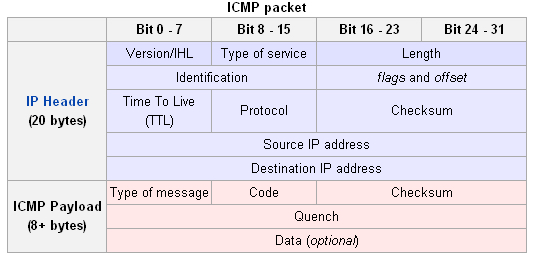
\includegraphics[width=\textwidth, bb = 0px 0px 535px 262px, keepaspectratio=true]{grafika/icmp_packet.jpg} 
	\caption{ Budowa pakietu ICMP. }
\end{figure}

Sposób ten ma jednak wiele wad, które w niektórych sytuacjach znacznie utrudniają lub wręcz uniemożliwiają jego wykorzystanie. Przedstawione zostały one poniżej:

\begin{itemize}
	\item Urządzenie monitorowane musi automatycznie odpowiadać na pakiety ICMP.
	\item Pakiety ICMP często mają bardzo niski priorytet i nie są powtórnie wysyłane po zagubieniu, powoduje to konieczność wysyłania pakietów do skutku, zaś jeden brak odpowiedzi na pakiet nie gwarantuje tego, że serwer jest niedostępny.
	\item Wiele serwerów, firewalli i urządzeń sieciowych takich jak routery i przełączniki blokuje całkowicie protokół ICMP w celu ochrony sieci.
	\item Wykorzystując pakiet ICMP (ping) można sprawdzić tylko dostępność urządzenia o podanym adresie IP w sieci – nie pozwala to na sprawdzenie dostępności konkretnego serwera zainstalowanego na danej maszynie.
\end{itemize}

\section{Istniejące rozwiązania.}

\begin{enumerate}
	\item Urządzenie monitorowane musi automatycznie odpowiadać na pakiety ICMP.
	\item Pakiety ICMP często mają bardzo niski priorytet i nie są powtórnie wysyłane po zagubieniu, powoduje to konieczność wysyłania pakietów do skutku, zaś jeden brak odpowiedzi na pakiet nie gwarantuje tego, że serwer jest niedostępny.
	\item Wiele serwerów, firewalli i urządzeń sieciowych takich jak routery i przełączniki blokuje całkowicie protokół ICMP w celu ochrony sieci.
	\item Wykorzystując pakiet ICMP (ping) można sprawdzić tylko dostępność urządzenia o podanym adresie IP w sieci – nie pozwala to na sprawdzenie dostępności konkretnego serwera zainstalowanego na danej maszynie.
\end{enumerate}

\section{Wymagania funkcjonalne}

Dawniej decyzja o wyborze pomiędzy istniejącym systemem operacyjnym a tworzeniem swojego oprogramowania od podstaw była skomplikowana i uwarunkowana bardzo często użytym sprzętem i potrzebami. Aktualnie, dzięki upowszechnieniu systemu Linux w systemach wbudowanych, ta decyzja bardzo często sprowadza się do wyboru jego dystrybucji i konfiguracji. Linux radzi sobie nawet w systemach czasu rzeczywistego od których wymagana jest wysoka wydajność \cite{ProLinuxEmbedded, AnalysisAndSynthesis}.

\section{Wymagania niefunkcjonalne}